%%% LaTeX Template
%%% This template can be used for both articles and reports.
%%%
%%% Copyright: http://www.howtotex.com/
%%% Date: February 2011

%%% Preamble

\documentclass[12pt,a4paper,twoside,norsk]{scrartcl}	% Article class of KOMA-script with 11pt font and a4 format
\usepackage{babel}														% English language/hyphenation
\usepackage[protrusion=true,expansion=true]{microtype}				% Better typography
\usepackage{amsmath,amsfonts,amsthm}										% Math packages
\usepackage[pdftex]{graphicx}														% Enable pdflatex
%\usepackage{color,transparent}													% If you use color and/or transparency
\usepackage[hang, small,labelfont=bf,up,textfont=it,up]{caption}	% Custom captions under/above floats
\usepackage{epstopdf}																	% Converts .eps to .pdf
\usepackage{subfig}																		% Subfigures
\usepackage{booktabs}																	% Nicer tables
\usepackage[utf8]{inputenc} % We want UTF8
\usepackage{url}
\usepackage{textcomp}

\usepackage{apacite}

%%% Advanced verbatim environment
\usepackage{verbatim}
\usepackage{fancyvrb}
\DefineShortVerb{\|}								% delimiter to display inline verbatim text

%%% Custom sectioning (sectsty package)
\usepackage{sectsty}								% Custom sectioning (see below)
\allsectionsfont{%									% Change font of al section commands
	\usefont{OT1}{bch}{b}{n}%					% bch-b-n: CharterBT-Bold font
%	\hspace{15pt}%									% Uncomment for indentation
	}

\sectionfont{%										% Change font of \section command
	\usefont{OT1}{bch}{b}{n}%					% bch-b-n: CharterBT-Bold font
	\sectionrule{0pt}{0pt}{-5pt}{0.8pt}%	% Horizontal rule below section
	}

%%% Custom headers/footers (fancyhdr package)
\usepackage{fancyhdr}
%\usepackage{tabularx}
\usepackage{float}
\pagestyle{fancyplain}
\fancyhead{}														% No page header
\fancyfoot[C]{\thepage}										% Pagenumbering at center of footer
\renewcommand{\headrulewidth}{0pt}				% Remove header underlines
\renewcommand{\footrulewidth}{0pt}				% Remove footer underlines
\setlength{\headheight}{13.6pt}

%%% Equation and float numbering
\numberwithin{equation}{section}															% Equationnumbering: section.eq#
\numberwithin{figure}{section}																% Figurenumbering: section.fig#
\numberwithin{table}{section}																% Tablenumbering: section.tab#
\newcommand{\HRule}{\rule{\linewidth}{0.5mm}} % command to make the lines in title page

%%% Glossary stuff
\usepackage[nonumberlist]{glossaries}
\newcommand{\dictentry}[2]{%
  \newglossaryentry{#1}{name=#1,description={#2}}%
  \glslink{#1}{}%
}
\makeglossaries

%%% Begin document
\begin{document}
\pagenumbering{Roman}
% This template from http://www.vel.co.nz

\begin{titlepage}

\begin{center}
 
% Upper part of the page

\textsc{\LARGE Norges Teknisk-Naturvitenskapelige Universitet}\\[1.5cm]

 
\textsc{\Large EIT3014}\\[0.5cm]

\textsc{\large En spillverden på ett semester}\\[0.5cm]
 
 
% Title
\HRule \\[0.4cm]
{ \huge \bfseries Prosjektrapport}\\[0.4cm]
 
\HRule \\[1.5cm]
 
% Author

\begin{center} \Large
\emph{Forfattere:}\\
Andreas Røysland \textsc{Aarnes}\\
Trond Kjetil \textsc{Bremnes}\\
Christian Aleksander \textsc{Lysne}\\
Kjetil \textsc{Mehl}\\
Ina Sander \textsc{Pedersen}\\ [3cm]
\end{center}
 
% Bottom of the page

{\large \today}\\[4cm] % \today inputs the current date, can be changed to any other date
 
\vfill
\end{center}

\end{titlepage}

\tableofcontents
% Add the chapters
\printglossary[style=list]
\addcontentsline{toc}{section}{Ordliste}
\dictentry{SNES}{
	Super Nintedo Entertainment System, Spillmaskin utgitt av Nintendo i 1992
}
\dictentry{Super Mario World}{
	Plattformspill utgitt av Nintendo til SNES i 1992
}
\dictentry{Nintendo 64}{
	Spillmaskin utgitt av Nintendo i 1996
}
\dictentry{Banjo Kazooie}{
	Platformspill til Nintendo 64, utgitt av Rare i 1998
}
\dictentry{Legend of Zelda}{
	The Legend of Zelda, en eventyrspillserie utgitt av Nintendo. Første spill til NES i 1986. Oppfølgeren The Legend of Zelda: Ocarina of Time, kanskje det mest populære spillet i serien, utgitt til Nintendo 64 i 1998
}
\dictentry{Fanboy}{Fanboy er et engelsk begrep som brukes for å beskrive et individ som
er dedikert til et enkeltobjekt på en emosjonell eller fanatisk måte,
ofte til et punkt der det kan beskrives som tvangslidelse
}
\dictentry{Energispillet}{
	Et energispill for å lære om energi, miljø og klima, utviklet av CyberLab
}
\dictentry{Advance Wars}{
	Strategispill orginalt utgitt til Game Boy Advance
}
\dictentry{Rayman}{
	En serie plattformspill orginalt utgitt og utviklet av Ubisoft
}
\dictentry{WC3}{
	Warcraft III, sanntidsstrategispill utgitt av Blizzard i 2002
}
\dictentry{Game Boy}{
	Benevnelse brukt om serien av handholdte konsoller utgitt av
Nintendo
}
\dictentry{DKC2}{
	Donkey Kong Country Country 2, et plattformspill til SNES, utgitt i 1995
}
\dictentry{SSBM}{
	Super Smash Brothers Melee, et slossespill, med de kjente Nintendo-figurene. Første spillet i serien utgitt til Nintendo GameCube i 2002
}
\dictentry{Diablo 2}{
	Et hack and slash action-rollespill, utgitt av Blizzard i 2000
}
\dictentry{Mario 64}{
	Det første Mario-spillet til Nintendo 64, utviklet og utgitt av
Nintendo i 1996
}
\dictentry{Mario Kart}{
	Mario Kart er en serie racingspill, med de kjente Nintendo-figurene.
Det første spillet kom til NES i 1992
}
\dictentry{Monkey Island}{
	Monkey Island, en serie med med eventyrspill i pek-og-klikk
sjangeren. Produsert av LucasArts
}
\dictentry{Den Lengste Reisen}{
	Eventyrspill laget og utgitt av norske Funcom i 1999
}
\dictentry{Bastion}{
	Et action-rollespill produsert av selskapet Supergiant Games. Ble sluppet i 2011 til Xbox Arcade, senere og til PC
}
\dictentry{Civilization}{
	Et turbasert strategispill i utgangspunktet utgitt til DOS i 1991. Ble
senere en serie og er nå i sin 5. generasjon
}
\dictentry{Starcraft}{
	Sanntidsstrategispill utgitt av Blizzard i 1998
}
\dictentry{C and C}{
	Command \& Conquer, strategispill først utgitt til PC
}
\dictentry{Tekken}{
	Et japansk kampsportspill utviklet av Namco og orginalt gitt ut til
Playstation
}
\dictentry{Wii}{
	Nintendo Wii, Nintendos siste spillkonsoll
}
\dictentry{NES}{
	Nintendo Entertainment System – 8 bits spillkonsoll utgitt av
Nintendo i 1986
}
\dictentry{GBA}{
	En av de håndholdte spillkonsollene utgitt av Nintendo i 2001
}
\dictentry{Xbox}{
	En serie spillkonsoller utgitt av Microsoft
}



\pagenumbering{arabic}
\section{Introduksjon}\label{sec:intro}
Dette avsnittet skal gi et kort overblikk over hvordan resten av
dokumentet er strukturert, hvilke spillmessige bakgrunner hver av
deltagerene i gruppen hadde, og hvilke mål som ble satt med tanke på å
utvikle et spillkonsept og en eventuell prototype.
\subsection{Struktur}
Dokumentet er i hovedsak strukturert i 4 hoveddeler:
\begin{enumerate}
	\item Introduksjon (Avsnitt~\ref{sec:intro})
	\item Konseptet (Avsnitt~\ref{sec:konsept})
	\item Utforming (Avsnitt~\ref{sec:design})
	\item Teknisk (Avsnitt~\ref{sec:teknisk})
\end{enumerate}
Konseptdelen skal gi en overordnet forståelse for hva spillet handler
om. Utformingdelen skal gi dypere innsikt i hvordan spillet er bygd opp,
og hvilke elementer det består av.
\subsection{Gruppemedlemmene}
Herunder vil den spillmessige bakgrunnen til hvert gruppemedlem bli
beskrevet.
\begin{description}
\item[Kjetil Mehl (23)] \hfill \\
Han begynte sin spillkarriere med en Nintendo 64\cite{n64} i 1999. Da
var det eventyr og rollespill (se Seksjon~\ref{sec:sjangre}) som Legend
of Zelda\cite{legendofzelda} og Banjo Kazooie\cite{banjokazooie} som
stod i fokus. Da datamaskinen kom i hus gikk spillfokuset  over på
konkurransespill som Counter-Strike og Warcraft. Han har i hovedsak vært
en Nintendo fanboy\cite{fanboy}, men har i de senere år utvidet
kolleksjonen til å omfatte Xbox.
\item[Ina Sander Pedersen (26)] \hfill \\
I 1996 oppdaget hun Rayman\cite{rayman} til PC og var fra den dag frelst for serien, men skiftet raskt konsoll til Playstation. For Ina har sjangeren plattform vært en klar favoritt gjennom årene og da hun senere fikk Gameboy Pocket\cite{gameboy} gikk tiden med til Donkey Kong Country 2\cite{DKC2}. Etterhvert som årene har gått har hun skiftet mellom Nintendo og Playstation, samt prøvd ut endel forskjellige sjangertyper, men Rayman og Donkey Kong seriene er og blir favoritter. 
\item[Christian Aleksander Lysne (22)] \hfill \\
Christian var 8 år da han fikk sin første Nintendo 64\cite{n64} , med spillene Super Mario 64\cite{mario64} og Mario Kart\cite{mariokart}. Senere gikk det i Legend of Zelda\cite{legendofzelda} og Super Smash Bros\cite{smash}. Tekken\cite{tekken} var også  populært i oppveksten. Warcraft 3\cite{wc3} og Diablo 2\cite{diablo2} tok etter hvert over, og spilles fortsatt i perioder.
\item[Andreas Røysland Aarnes (25)] \hfill \\
Som seksåring prøvde Andreas Super Mario World\cite{supermarioworld} på Super Nintendo\cite{supernintendo} for første gang, og det var ikke før i 2011, da remaken New Super Mario Bros. Wii\cite{newsupermario} kom til Nintendo Wii\cite{wii}, at han igjen ble tilfredstilt innen spillverdenen. I mellomtiden har han låst seg til strategispill-seriene Warcraft\cite{wc3}, Command \& Conquer\cite{cc} og Age of Empires\cite{aoe}. 
\end{description}
\subsection{Mål}
Det overordnede målet for gruppen var å lage et spillkonsept hvert
gruppemedlem følte eierskap til, og var konformt med den valgte
problemstillingen (se Seksjon~\ref{sec:problemstilling}). En prototype i
tillegg til dette ville bli en bonus i forhold til målet.
\subsection{Prosessen}
Dette avsnittet forteller hvordan konseptet ble til ved å gå fra en
problemstilling, til en idè og til slutt et konsept. Den første delen av
denne prosessen var ikke iterativ, ettersom gruppen i praksis gikk fra
en vagt definert problemstilling, til en idè, for så å redefinere ideen
for å bedre passe den valgte problemstillingen. Prosessen gikk deretter
fra idè til konsept.
\subsubsection{Fra problemstilling til idè}
Det ble brukt mye tid på å utforske forskjellige ideer som var
interessante. Gruppen følte seg ikke veldig bundet av den opphavlige
problemstillingen, og eksperimenterte derfor med forskjellige ideer.
Gitt problemstillingen i Avsnitt~\ref{sec:problemstillingen} var det
naturlig å tenke på et spill som var turbasert eller sanntidsspill med
flere spillere. Etter flere runder internt ble det enighet rundt
følgende idè.
\begin{description}
\item[Energispillet med flerspillermodus] \hfill\\
Spillere skal organisere hver sin lille by, hvor fokuset er å forhandle
med hverandre på grunnlag av hvilke energitype de forskjellige byene
velger å gå for. En by som for eksempel fokuserer på kull kan raskt få
mye resurser, men ville påvirke sitt eget miljø lokalt, og senere hele
miljøet globalt.
\end{description}
Etter tilbakemeldinger fra landsbylederen viste deg seg derimot at ideen
ikke samsvarte godt nok med problemstillinga som var valgt. Dette førte
til restrukturering av den opphavlige ideen, for å få mer fokus på
gjenbruk og resirkulering. Følgende elementer fra ideen ble tatt med
videre:
\begin{itemize}
	\item Flerspiller
	\item Hver spiller har en base
	\item Bruk av søppel som ressurser, istedenfor energi
	\item Lokale faktorer kan påvirke det globale miljøet
\end{itemize}
\subsubsection{Redefinering av ideen}
Den opphavlige ideen skle over på å bli et rent konkurransespill, med
mindre fokus sanking/utvinning av resurser. For å minske ressursfokuset
ble det bestemt at hver øy er en ``søppeløy'', og målet til spilleren er
å fjerne alt søppelet på sin øy.  Ressurser blir utvinnet ved å
resirkulere søppelet på øya. Ved å legge inn denne vrien ble ideen mer
konformt med problemstillingen. 

%Det ble gjort koblinger opp mot et spill lignende Advanced
%Wars\cite{advancewars} eller Wordfeud\cite{wordfeud} med fokus på
%miljøet.

\section{Problemstilling}\label{sec:problemstilling}
Dette avsnittet vil ta for seg den valgte problemstillingen, hva som lå
til grunn dette valget, og hvordan gruppen tenkte seg et konsept rundt
problemstillingen.
\subsection{Selve problemestillingen}
Den valgte problemstillingen er gjengitt nedenfor:
\begin{quotation}
\large\emph{``Hvordan kan en belyse nytten av resirkulering og redusert forbruk,
lokalt og globalt, gjennom flerspiller-dataspill
''}
\end{quotation}

\section{Prosessen}
Dette avsnittet forteller hvordan konseptet ble til ved å gå fra en
problemstilling, til en idè og til slutt et konsept. Den første delen av
denne prosessen var ikke iterativ, ettersom gruppen i praksis gikk fra
en vagt definert problemstilling, til en idè, for så å redefinere ideen
for å bedre passe den valgte problemstillingen. Prosessen gikk deretter
fra idè til konsept.
\subsection{Fra problemstilling til idè}
Det ble brukt mye tid på å utforske forskjellige ideer som var
interessante. Gruppen følte seg ikke veldig bundet av den opphavlige
problemstillingen, og eksperimenterte derfor med forskjellige ideer.
Gitt problemstillingen i Avsnitt~\ref{sec:problemstillingen} var det
naturlig å tenke på et spill som var turbasert eller sanntidsspill med
flere spillere. Etter flere runder internt ble det enighet rundt
følgende idè.
\begin{description}
\item[Energispillet med flerspillermodus] \hfill\\
Spillere skal organisere hver sin lille by, hvor fokuset er å forhandle
med hverandre på grunnlag av hvilke energitype de forskjellige byene
velger å gå for. En by som for eksempel fokuserer på kull kan raskt få
mye resurser, men ville påvirke sitt eget miljø lokalt, og senere hele
miljøet globalt.
\end{description}
Etter tilbakemeldinger fra landsbylederen viste deg seg derimot at ideen
ikke samsvarte godt nok med problemstillinga som var valgt. Dette førte
til restrukturering av den opphavlige ideen, for å få mer fokus på
gjenbruk og resirkulering. Følgende elementer fra ideen ble tatt med
videre:
\begin{itemize}
	\item Flerspiller
	\item Hver spiller har en base
	\item Bruk av søppel som ressurser, istedenfor energi
	\item Lokale faktorer kan påvirke det globale miljøet
\end{itemize}
\subsection{Redefinering av ideen}
Den opphavlige ideen skle over på å bli et rent konkurransespill, med
mindre fokus sanking/utvinning av resurser. For å minske ressursfokuset
ble det bestemt at hver øy er en ``søppeløy'', og målet til spilleren er
å fjerne alt søppelet på sin øy.  Ressurser blir utvinnet ved å
resirkulere søppelet på øya. Ved å legge inn denne vrien ble ideen mer
konformt med problemstillingen. 
\begin{description}
\item[Garbarge Alert] \hfill\\
Spillerene skal organisere hver sin lille søppelfylt øy. Målet er å
fortest mulig kvitte seg med søppelet på sin øy. Dette kan bli gjort ved
resirkulering, eller ved å sabotere for de andre spillerene ved å flytte
ditt søppel over til dem. Utifra aksjonene til de forskjellige
spillerene kan både lokale og globale katastrofer inntreffe. Spilleren
som først rydder sin øy, eller som står igjen til sist vinner spillet.
\end{description}
Utifra denne korte beskrivinga begynte vi å arbeide opp mot et konkret
konsept, som beskrevet i Avsnitt~\ref{sec:konsept}.
%Det ble gjort koblinger opp mot et spill lignende Advanced
%Wars\cite{advancewars} eller Wordfeud\cite{wordfeud} med fokus på
%miljøet.

\cleardoublepage
\section{Konseptet}\label{sec:konsept}
Målet med dette avsnittet er å gi et innblikk i det utviklede konseptet,
hvilke spillaspekter som er tatt med og spilldynamikken.

Garbage Alert er et sanntids strategispill for mobile enheter. Hver
spiller blir tildelt en øy dekket med søppel. En øy består av en
gjenvinningsstasjon, en våpenstasjon og en forsvarssone.
Gjenvinningsstasjonen har som oppgave å transformere øyas søppel om til
ressurser. Disse ressuresene kan brukes til å kjøpe våpen,
forsvarsmurer, utvinne nye ressurser og oppgradere
gjennvinningsstasjonen. Mulige oppgraderinger for gjenvinningsstasjonen
er raskere gjennvinning og større kapasitet for inntak av søppel. Våpen
brukes til å skyte søppel på motstandernes øyer, og forsvarsmuren har
som oppgave å blokkere slike angrep. 

Det er flere muligheter for å vinne i dette spillet. Det første
vinnsenarioet er å bli den første til å kvitte seg med alt søppelet på
øyen sin. Den andre måten å vinne på er å skyte i stykker motstandernes
gjenvinningsstasjon. Hvis en øy mister gjenvinningsstasjonen sin, vil
den bli oversvømt med søppel og synke ned i havet. Dermed kan spilleren
velge om han/hun vil fokusere på å forbedre sin egen øy eller ødelegge
for andre. 

\section{Spillutforming}\label{sec:design}
Denne seksjonen tar for seg hvordan spillet i helhet er utformet.
Definisjonene spillet bruker blir forklart, spilldynamikken blir updypet,
og de forskjellige spillelementene blir beskrevet.
% This is a section where the definition of the game play is established.
% Definitions should include how a player wins, loses, passes levels and
% the main focus of the game play.
\subsection{Definisjoner}
Dette avsnittet forklare de grunnleggende definisjonene rundt Garbage
Alert. Definisjonene er i hovedsak sentrert rundt hvordan spilleren
oppfatter spillet~\cite{gameplay}.
\subsubsection{Oppstart}
Alle spillere starter med like forutsetninger. Hvordan spillet utvikler
seg kommer an på hvordan spillerene bruke ressursene som er gitt.
\subsubsection{Vinning}
En spiller har vunnet dersom alle de andre spillerene har mistet
gjenvinningsstasjonene sine, eller spilleren klarer å blit kvitt alt
søppelet på sin øy.
\subsubsection{Taping}
En spiller taper dersom gjenvinningsstajonen dens blir ødelagt. Spilleren
vil også tape dersom en annen spiller klarer å renske sin øy for søppel.


% This is a spreadsheet containing the generic names of the player and
% antagonistic elements and their game properties. 

% This should allow an easy cross reference for an elements in the game
% that a value. 
\subsection{Spillmatrisen}
Spillmatrisen (se Figur~\cite{fig:spillmatrise}) er en grafisk forklaring
på hvilke elementer i spillet som interagerer med hverandre. Elementer
som våpen, forsvar og oppgraderinger er kun beskrevet på et overordnet
nivå, siden disse elementene deler like egenskaper (f.eks. at alle
angrep kan angripe forsvar).
\begin{center}
\begin{figure} [H]
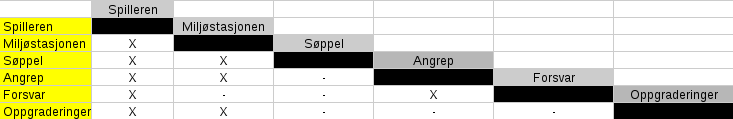
\includegraphics[scale=0.6]{images/spillmatrise.png}
\label{fig:spillmatrise}
\caption{Spillmatrise med de forskjellige elementene}
\end{figure}
\end{center}
I Figur~\cite{fig:spillmatrise} er elementene som interagerer er merket
med en \textbf{X} i den kollonnen og raden de elementene sammenfaller i.
Hvordan elementene interagerer er beskrevet nedenfor:
\begin{description}
\item \textbf{Spilleren}\\Spilleren sin oppgave er å samle søppel,
bygge våpen og forsvar, samt oppgradere miljøstasjonen.
\item \textbf{Miljøstasjonen}\\Miljøstasjonen tar imot og gjenvinner
søppelet. I tillegg er dette hovedbasen for spilleren, og står for alle
oppgraderingene. En miljøstasjon kan bli angrepet av andre spillere, og
interagerer derfor med våpen.
\item \textbf{Søppel}\\Blir plukket opp av spilleren, og lagt på
miljøstasjonen for gjenvinning.
\item \textbf{Angrep}\\Spillere kan angripe andre spillere sitt forsvar,
og miljøstasjonene deres.
\item \textbf{Forsvar}\\Forsvaret kan bli angrepet og ødelagt av våpen.
En spiller bygger forsvaret, derfor koblingen mellom spiller og forsvar.
\item \textbf{Oppgraderinger}\\Spilleren kan oppgradere miljøstasjonen
sin. Desse oppgraderingene baserer seg på statusen til miljøstasjonen.
\end{description}


% List all the elements that are directly related to or to the benefit
% of the player.

% Devise two sets of names for player elements. One set is a generic name
% (or code) and the other is its game name. 

% Describe the terminology that you use to describe the player’s
% properties.

%bruk ord: MILJØSTASJON, GJENVINNING. (ikke gjenvinningstasjon, utvinne, resirkulering)

\subsection{Elementer}
Dette avsnittet forteller om de forskjellige spillelementene som finnes
i Garbage Alert.
\subsubsection{Ressurser}
Ressurser er et viktig element i Garbage Alert. Ressursene er det som
gjør at spillere kan utvikle basen sin, bygge forsvar og utvikle angrep.
Valget av ressurser er basert på Mohs hardhetsskala av mineraler \cite{mohs}. Mohs hardhetskala er en liste over mineraler i rekkefølge etter absolutt hardhet, laget av geologen Friedrich Mohs. Hvert mineral skal kunne skrape mineralet som står foran på listen. Ressursene i Garbage Alert er ikke helt korrekte i forhold til Mohs hardhetsskala, men basert på denne. Idèen er at hver de seks ressursene i spillet følger samme regel, nemlig at den ene ressursen er hardere enn den andre og har mulighet til å ødelegge den. 
De forskjellige typene utvinnbare ressurser er:
\begin{description}
	\item \textbf{Papp}\\ Denne ressursen kan utvinnest uten å måtte
oppgradere miljøstasjonen. Dette er den enkleste ressursen å få fatt i,
men skaper kun relativt svake angrep/forsvar.
	\item \textbf{Plast}\\ Denne ressursen kan man utvinne etter å ha
oppgradert hovedbasen èn gang.
	\item \textbf{Tre}\\ Tre kan utvinnest dersom hovedbasen har blitt
oppgradert til dette. Tre er på samme oppgraderingsnivå som plast, med andre ord må
spilleren velge mellom desse to i begynnelsen. Tre er derimot hardere enn plast i dette spillet.
	\item \textbf{Jern}\\ Jern er mulig å utvinne dersom spilleren først
oppgraderer til tre.
	\item \textbf{Stål}\\ Stål bygger på at spilleren først har
oppgradert til plast.
	\item \textbf{Titan}\\ Titan er den siste ressursen som er mulig å
utvinne. For å kunne utvinne titan må spilleren først ha skaffet seg
alle utvinningsutvidelsene til hovedbasen.
\end{description}


Det er også mulig å skade forsvar/våpen som er bygget av en bedre ressurs enn våpenet. Dette er implementert slik at ingen våpen/forsvar blir uovervinnelige. Figur \ref{fig:ressursoppgraderinger} framstiller hvilke utvidelser man må ha for å kunne oppgradere til neste nivå. Allerede helt fra starten av spillet må man velge om man først vil oppgradere til tre, eller til plast (se seksjon \ref{miljostasjon}). 

	\begin{figure} [H]
				\begin{center}
					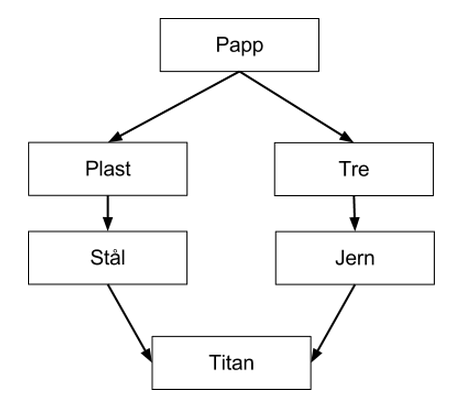
\includegraphics[scale=0.5]{images/oppgraderingstre}
				\end{center}
			\caption{Ressursoppgraderinger}
			\label{fig:ressursoppgraderinger}
	\end{figure}

\subsubsection{Ressursutvinning}
En spiller skaffer seg ressurser ved å gjenvinne søppel som ligger
spredt rundt på øya. Dette blir gjort ved hjelp av miljøstasjonen
som hver spiller starter med.
\subsubsection{Miljøstasjon} \label{miljostasjon}
Miljøstasjonen er det mest sentrale spillelementet i Garbage
Alert. Denne kan bli sett på som hovedbasen i spillet.
Miljøstasjonen kan oppgraderes på tre måter for å forbedre effektiviteten:\\
\begin{description}
	\item \textbf{Volum/Utvinningsgrad}\\Denne oppgraderingen kan øke utvinningsgraden og volumet av søppel som blir brukt i gjennvinningsprosessen. Restavfallet (søppelet som ikke blir gjenvunnet) vil på magisk vis bli borte. Tabell \ref{tab:effektivitet} viser oppgraderingene for Volum/Utvinningsgrad. Man starter på nivå 0, og deretter kan man oppgradere ett trinn ad gangen.
	\item \textbf{Buffer}\\Miljøstasjonen kan få en buffer hvor spilleren kan samle opp søppel, som automatiserer gjenvinningsprosessen til en viss grad. Dermed kan spilleren bruke mindre tid på å sørge for at søppelet på øyen blir flyttet til miljøstasjonen.
	\item \textbf{Ressurser}\\For å kunne gjenvinne nye typer ressurser må
		spilleren oppgradere gjenvinningsstasjonen. Her får spilleren valget
		mellom to ulike veier som vil avgjøre hvilke ressurser spilleren får
		tilgang til (se figur \ref{fig:ressursoppgraderinger}).
\end{description}

\begin{table} \label{tab:effektivitet}
\begin{tabular}[\textwidth]{ l  l  p{3cm}  l  p{4cm} } %\label{tab:effektivitet}
\hline
\bf{Effektivitet} & \bf{Utvinningsgrad} & \bf{Volum} & \bf{Tid} & \bf{Ressurskrav} \\
\hline
Nivå 0 & 10 & 10 & 15sek & Ingen  \\
Nivå 1 & 20 & 10 & 15sek & Papp \\
Nivå 2 & 30 & 10 & 15sek & Papp, og plast eller tre \\
Nivå 3 & 30 & 20 & 15sek & Papp, plast, tre, stål, jern og titan \\
\hline
\end{tabular}
\caption{Oppgraderinger for Volum/Utvinningsgrad}
\end{table}




\subsubsection{Forsvar}
Spillere kan bygge forsvar rundt øya si. Dette forsvaret vil forhindre
motspillere å angripe gjenvinningsstasjonen. Det vil finnes ulike typer
forsvarsmurer, som er kraftige/svake mot ulike typer angrep.
\subsubsection{Angrep}
En spiller får utdelt tre angrepsplattformer. På desse tre platformene
kan spilleren velge hvilke angrep han vil utvikle, basert på hvilke
tilgjengelige ressurser han har.
\subsubsection{Oppgraderinger}
Spilleren har mulighet til å oppgradere både gjenvinningsstasjonen,
våpen og forsvar. Hver type våpen og forsvar har tre nivå, der øking i
nivå vil gi hhv. kraftigere angrep og sterkere forsvar. De tre
våpenplassene på øya kan ha inneholde ulike våpen som kan oppgraderes
hver for seg.
Eksempel på forsvarsoppgradering:\\
Tremur (nivå 1) -> Tremur (nivå 2) -> Tremur (nivå 3).
\begin{quote}
Bør restruktureres!!\\
Spilleren kan utvinne ressurser ved å "dra" søppelenheter fra
forskjellige plasser på øya inn til gjennvinningsstasjonen. Hvilke
ressurser, og mengden av hver ressurs, som spilleren får ut fra en
enkelt søppelenhet er avhengig av nivået på gjennvinningsstasjonen og
hvilke typer oppgraderinger som er gjort. Spilleren kan også bruke sine
våpen til å bli kvitt søppelenheter. Her vil ubehandlede søppelenheter
kunne skytes på motstandere. Effekten av angrepet avhenger av spillerens
våpen, oppgraderingsnivå på våpenet og motstanderens forsvar. For å
beskytte seg mot angrep kan spilleren bygge mur rundt sin øy. Hvilke
våpen og forsvarsmurer som spilleren kan bygge er avhengig av hvilke
ressurser gjenvinningsstasjonen er i stand til å utvinne. Dette betyr at
valg av typer oppgradering for gjenvinningsstasjonen vil være avgjørende
for utviklingen av spillet.\\
\end{quote}

% Make a list of all objects that affect the player in a positive way.
% (i.e. health replenished)

% Define these objects by describing what affect they cause and how the
% player can use the object.
\subsection{Spillerpremier}

Gjennom å oppgradere ens miljøstasjon vil en kunne visuelt se at øya blir renere, atmosfæren blir klarere og bakgrunnsmusikken blir penere. Lystige lydeffekter signaliserer at en gjør noe som gir spilleren en fordel i forhold til motspillerne, for eksempel når en oppgraderer ens utstyr eller utfører et vellykket angrep mot sine motstandere. Dette håper vi skaper en positiv følelse av mestring hos spilleren. 

Videre er der en intrisitt verdi i å vinne et spill over ens medspillere.

For å kunne underbygge spillets underliggende tematikk om miljøvennlighet vil naturen straffe spillerne om de er er for miljøuvennlige med naturkatastrofer.

På samme måte som at muntre lydeffekter underbygger gode handlinger gjort av spilleren, vil dystre lydeffekter signalisere negative hendelser. Dette kan for eksempel være i det en blir angrepet av motspillerne. 
% This is where a description of the user’s control of the game can be
%placed.

% It is also recommended to think about which buttons on a device would
% be best suited for the game.

% Consider what the worst layout is, then ask you self if your UI is it
% still playable?

% A visual representation can be added, where we relate the physical
% controls to the actions in the game.


% TODO
% * Skrive om de svakeste elementene i grensesnittet
% * Referere til screenshots
% * Inkludere noe tekst om lydbildet?
% * Generell formattering, sammenslåing og sortering av avsnitt

\subsection{Brukergrensesnitt}



Brukergrensessnittet i spillet er i prototypen noe infantilt og uferdig.


Vi har bevisst valgt å holde språket i spillet norsk, og overalt hvor en finner tekst i spillet vil den være på norsk. % bah, møkkasetning.


Det en først ser når en starter spillet er en introskjerm som med sin grafikk og lydbilde er ment å sette spilleren i et kompetetivt sinnelag.

Fra denne skjermen er det mulig å starte spillet ved å trykke den store knappen markert "Start".
En mer ferdig versjon vil andre valg fra denne skjermen være å stille inn ting som spillernavn, samt mulighet for å koble flere spillere sammen i et flerspillerspill.


Spillets hovedskjerm % Forklare litt bedre hva vi mener med hovedskjerm
består av et overblikksbilde av alle øyer som er med i spillet. I prototypen er antallet begrenset til to, men en mer moden versjon vil inneholde muligheten til å spille flere enn to stykker samtidig. En skiller mellom en selv og andre ved bruk av ulike farger på spillernes miljøstasjon, våpen og forsvar. I prototypen har vi valgt å fargelegge de to faksjonene rød og blå.

I prototypen er denne skjermen et statisk fugleperspektiv av alle øyene og alle spillets elementer. En ferdig versjon vil og inneholde muligheten til å veksle mellom et detaljbilde av ens egen øy og overblikksbildet over alle øyer. Hvorvidt dette vil gjøres via en knapp som veksler mellom de to visningsmodi eller om en vil "klype for å zoome" er på dette stadiet uvisst og bør testes via brukertesting for å finne den optimale metoden.


Garbage Alert er tenkt å først og fremst spilles på mobiltelefoner og andre enheter med berøringsskjerm. En interagerer derfor med elementene på skjermen ved å trykke på de. Det en må være spesielt oppmerksom på med slike skjermer er å holde knapper store nok, samt at aller elementer på skjermen må være forskjellige nok til at det er enkelt å skille de fra hverandre på små skjermer.

Spillet kan og spilles på en datamaskin i en nettleser, og en kan derfor også bruke en musepeker for å trykke på elementene på samme måte.


Merk at da vi under utviklingen kun har testet prototypen på en dataskjerm er ikke spillet per nå tilpasset mobiltelefoner i så stor grad som det burde være. Enkle tester på mobiltelefon har dog blitt gjort, men har vært nedprioritert grunnet tidspress.


\cleardoublepage
%!TEX root = report.tex
\section{Teknisk utførelse}\label{sec:teknisk}
Denne seksjonen vil detaljere hvordan Garbage Alert per i dag er
implementert, samt tanker om videre utvikling til en eventuell ferdig
versjon.
\subsection{Tidlig prototype}
Tidlig i prosessen ble det utviklet en enkel web-basert prototype som
kunne brukes for å utforske spillets dynamikk. Denne var hjelpsom for å
fastslå hvilke deler av konseptet som fungerte, og ikke fungerte. Se
figur~\ref{fig:screenshot_tidlig_prototype}, under for et skjermskudd av
denne prototypen. Et mål var å ha noe som fungerte, men samtidig
realisere den med minimal bruk av tid.
\begin{figure} [H]
	\begin{center}
	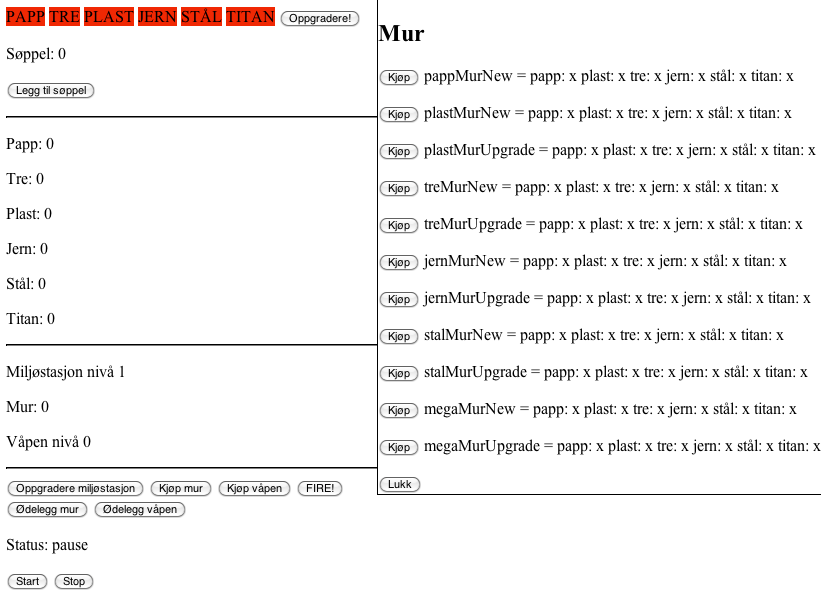
\includegraphics[scale=0.3]{images/screenshot_tidlig_prototype.png}
	\end{center}
	\caption{Skjermskudd av vår tidlige prototype}
	\label{fig:screenshot_tidlig_prototype}
\end{figure}

Denne programkoden, sammen med penn, papir og en solid dose fantasi
gjorde oss i stand til å spille spillet sammen på et veldig tidlig
stadie, noe som gjorde oss i stand til å gjøre nødvendige justeringer
for å gjøre spillet morsommere å spille. Vi kunne og gjøre et bedre
anslag på spillets ressurskostnader og
nedkjølinger\footnote{Nedkjølinger er et ord som benyttes om den tiden
det tar fra du utfører en handling til du får lov til å utfører den
igjen.}.

Denne prototype-koden ble og senere mye brukt, sammen med en bedre grafisk presentasjon, for å realisere den endelige protoypen.



\subsection{Endelig prototype}

Garbage Alert-prototypen slik den er i dag er implementert med de nye
web-teknologiene (noe unøyaktig) kjent som HTML5. Mer nøyaktig vil dette si at spillet er implementert med et \texttt{<canvas>} element, et lite "malebrett" som en kan tegne på programmatisk med JavaScript. Dette medfører at Garbage Alert i prinsippet kan kjøres hvor som helst der en har en moderne nettleser med støtte for JavaScript. Garbage Alert har moderne berøringsbaserte mobiltelefoner som hovedplattform, hvor slik teknologi kjører uten problemer.





Enkelte av elementene er dog implementert via andre ymse metoder, som for eksempel hvite overlegg som ser litt malplassert ut i forhold til resten av grensesnittet, grunnet gjenbruk av kode fra en tidligere prototype, for å raskt kunne iterere og skape en prototype vi kunne teste ut og vise fram. Dette ville i en ferdig versjon blitt implementert på en skikkelig måte.


\subsubsection{Systemkrav}
Som nevnt over er Garbage Alert først og fremst ment å kunne spilles på mobiltelefoner.
Da spillet er implementert som et web-basert spill vil det i prinsippet ikke være en begrensning på hvilket operativsystem telefonen kjører, det være Apple iOS, Google Android eller Windows Phone 7, så lenge telefonen leveres med en moderne nettleser. Nettbrett som Apple iPad og Samsung Galaxy Tab vil og kunne kjøre Garbage Alert.

I tillegg til dette vil spillet kunne spilles ellers hvor der finnes moderne/kompatible nettlesere. Det store aberet her er at kontrollmetoder ikke alltid vil fungere optimalt, og må eventuelt tilpasses de ulike plattformers styrker og svakheter. Slik prototypen eksisterer i dag vil den eksempelvis fungere bra med mus og tastatur på en tradisjonell datamaskin, men ikke i det hele tatt med en styrespak.

Legg dog merke til at ekstensiv testing av ulike nettlesere og enheter har ikke blitt gjort, og gruppen kan ikke gå god for at spillet kjører feilfritt over alt. Garbage Alert er hovedsaklig testet i Google Chrome (versjon 18 og over) og Opera (versjon 11.6 og over). Spillet har blitt testet noe på mobiltelefoner, men ikke ut over det å sikre at spillet fungerer \emph{greit}. I en endelig versjon må grensesnittet tilpasses bedre, og ekstensiv testing måtte vært utført for å sikre at spillet fungererer skikkelig.


\subsubsection{Audiovisuelt innhold}
Garbage Alerts visuelle stil er ment å være leken og samtidig
oversiktlig, og dets grafiske stil er inspirert av den klassiske
spillserien Advance Wars.

Spillets introskjerm er ment å være så pompøs og lite subtil som mulig,
med store eksplosjoner på en søppelhaug. På denne skjermen spilles et
utsnitt av sangen \emph{Hell March}, kjent som tittelmusikken fra
Westwoods Red Alert-serie. Dette for å underbygge det pompøse inntrykket
vi ønsker å skape. En ferdig versjon vil inneholde lydeffekter og
bakgrunnsmusikk i resten av spillet.

En mer fullstendig utdyping av spillets audiovisuelle innhold finnes i
seksjon \ref{sec:artwork}.



\subsubsection{Programmeringsinnhold og kodestruktur}
Som nevnt over er spillet programmert i JavaScript fra grunnen av uten hjelp av eksisterenede hjelperammeverk. Dette er dels fordi implementasjonen av spillet er tenkt å være enkel, samt at slike rammeverk er noe umodne.
Logisk kodestruktur og -arkitektur har ikke vært noe som har blitt tenkt mye på, og kun enkle grep har blitt gjort for å gjøre koden noe enklere å skrive. Dette gjelder spesielt den koden som har blitt arvet fra den tidligere prototypen, kode som med god grunn kan omtales som et "lappeteppe".

For å øke spillets modifiserbarhet og øke kodens lesbarhet er de ulike elementene i spillet delt inn i egne JavaScript-filer for å logisk samle metoder og funksjoner. I en ferdig versjon vil disse filene samles i én enkelt fil for å gjøre eksempelvis innlastingstiden bedre.

Spillets bilder og figurer finnes i en egen mappe. På samme måte som med JavaScript-filene vil en i den ferdige versjonen ha salle bildene i én større bildefil for å forbedre innlastingstiden.


\subsubsection{Problemer og alternativer}
Da vi har sett oss ut berøringsbaserte mobiltelefoner som målplattform for spillet vil de naturlige alternativene være å realisere Garbage Alert som en såkalt \emph{native} applikasjon\footnote{En \emph{native} applikasjon er en skreddersydd applikasjon skrevet direkte til ett enkelt av de ulike mobiltelefonoperativsystemene.}, noe vi også til å begynne med hadde tenkt å gjøre. Dette gikk vi imidlertid bort fra da ikke alle har de verktøy som behøves for å utvikle til denne plattformen\footnote{Der behøves en Apple Mac og en utviklerlisens, noe kun ett menneske på gruppa har.} falt valget med hvert på å implementere spille med web-teknologi. Dette førte med seg at flere kunne bidra til programmeringen både i kraft av at flere har erffaring med JavaScript fra før og at alle er i besittelse av de verktøy som behøves.

Spill skrevet i JavaScript vil være tregere enn spill skrevet native, men dette er noe vi har valgt å se bort fra. Dette fordi en enkel prototype vil fungere tilstrekkelig i dette prosjektet.

Det som nevnt ingen garanti at spillet vil fungere i alle nettlesere overalt, og ekstensiv testing må til for å kunne sikre at det fungerer på flest mulig enheter. Igjen, grunnet at resultatet av dette prosjektet var ment å kun være en enkel prototype, er dette noe vi har sett bort fra.

Flerspiller-delen av spillet har ikke blitt implementert, ei heller en kunstig intelligens til motspilleren.


\subsubsection{Ressurser}
Garbage Alert kan utvikles i hvilken som helst applikasjon som er i stand til å redigere rene tekstfiler. Kildekontroll gjøres via Git, og koden er lagret på GitHub\footnote{\url{https://github.com/aspic/Garbage-Alert}}. Spillet kan og spilles fra spillet nettside på \url{http://aspic.github.com/Garbage-Alert}.

\subsubsection{Hvordan spille Garbage Alert lokalt}
Forutsett at du har Git og Python\footnote{Hvilken som helst server-programvare kan benyttes, Python nevnes her da dette verktøysettet er temmelig utbredt og er enkelt å starte.} installert, her er hvordan du starter spillet fra egen datamaskin via en terminalklient.

Først, last ned kildefilene fra GitHub med kommandoen \newline\texttt{git clone git://github.com/aspic/Garbage-Alert.git}. Spillet vil da lastes ned til mappen \texttt{Garbage-Alert}. Navigér til mappa kalt \texttt{webver} under denne  og start spillet med kommandoen \texttt{python -m SimpleHTTPServer 8080}. Start en kompatibel nettleser og navigér til URLen \url{http://localhost:8080}. Garbage Alert vil nå kjøre lokalt på din datamaskin.

\cleardoublepage
%!TEX root = report.tex
\section{Grafisk fremstilling}\label{sec:artwork}
Under vil den grafiske fremstillingen av \emph{Garbage Alert} bli beskrevet
sammen med valgene som har blitt gjort. Dette vil illustreres med
skjermskudd.

Den grafiske fremstillingen i spillet er ment å være leken og rettet mot
barn i alle aldre, og er sterkt inspirert av den klassiske spillserien
Advance Wars. Videre har det å holde ting oversiktlig og stort nok til å
trykkes på en berøringsskjerm vært noe vi har hatt spesielt i tankene
når grensesnittet har blitt utformet. Det er lagt mer vekt på
funksjonalitet, enn selve fremstillingen på denne delen av stadiet. Av
skjermskuddene ser en to forskjellige spillere som spiller mot
hverandre.

Som en ser av figur~\ref{fig:Oppgradering} kan spilleren på dette
tidspunktet kun oppgradere til plast. Dette er med andre ord i en tidlig
fase av spillet. Tilgjengelige ressurser er vist i bunnen av
skjermskuddet, og på dette tidspunktet kan miljøstasjonen kun gjenvinne
plast.

På figur~\ref{fig:Eksplosjon} har den blå spilleren angrepet den røde
spilleren, og man ser effekten av dette i eksplosjonen.

\begin{figure} [H]
\centering
\setlength\fboxsep{0.2pt}
\setlength\fboxrule{0.7pt}
\fbox{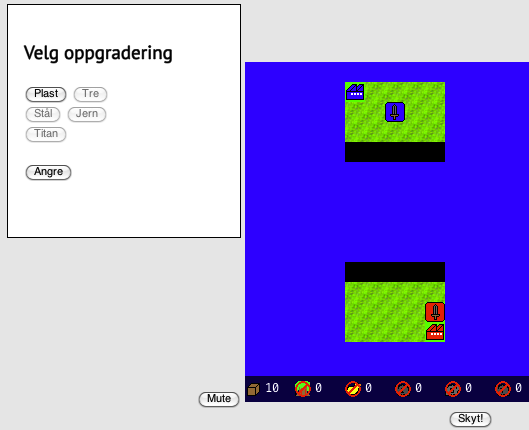
\includegraphics[width=\textwidth]{images/Oppgradering.png}}
\caption{Miljøstasjonen kan oppgraderes til å håndtere ulike typer avfallsgjenvinning.}
\label{fig:Oppgradering}
\end{figure}

\begin{figure}
\centering\setlength\fboxsep{0.2pt}
\setlength\fboxrule{0.7pt}
\fbox{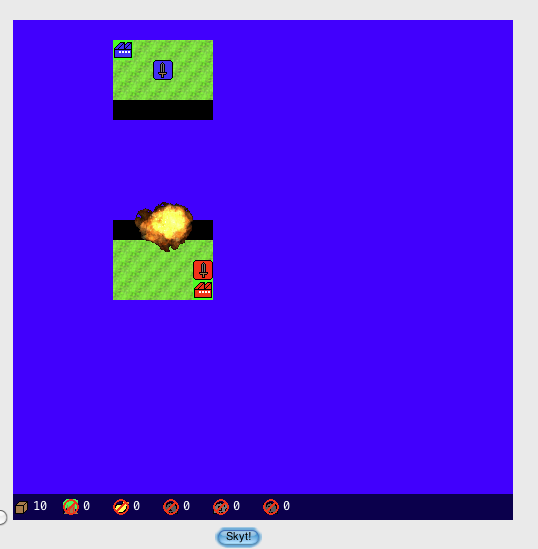
\includegraphics[scale=0.5]{images/Eksplosjon.png}}
\caption{Ved et angrep på en annen spiller vil et projektil avfyres og eksplodere på motspillerens eventuelle forsvarsstruktur.}
\label{fig:Eksplosjon}
\end{figure}

\begin{figure}
\centering
\setlength\fboxsep{0.2pt}
\setlength\fboxrule{0.7pt}
\fbox{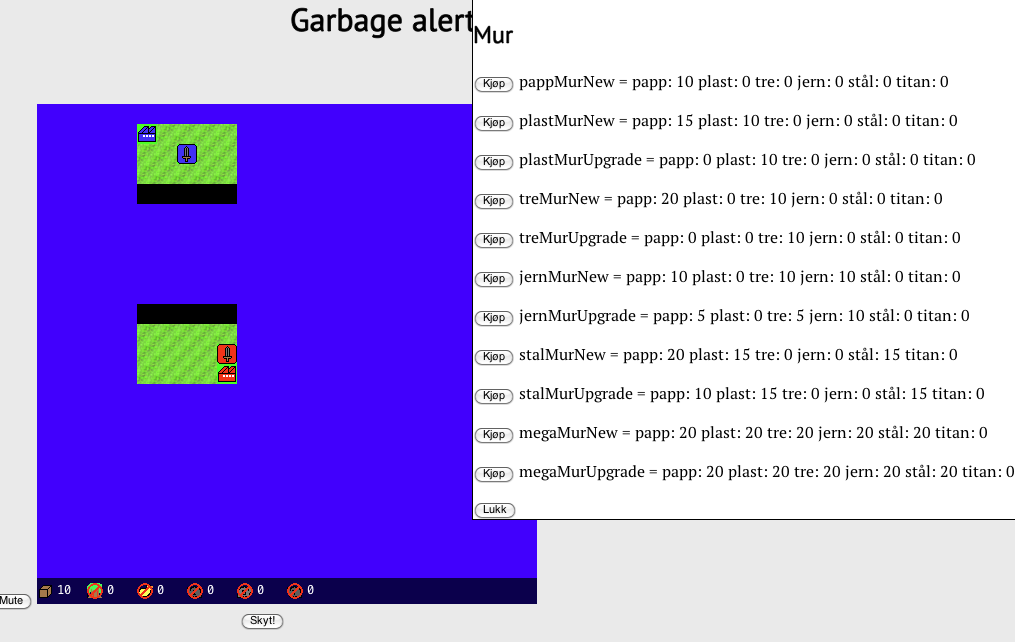
\includegraphics[width=\textwidth]{images/OppgradereMur.png}}
\caption{Spillerens forsvarsstruktur kan oppgraderes til å håndtere sterkere skyts fra motspilleren, avhengig av tilgjengelige ressurser.}
\label{fig:OppgradereMur}
\end{figure}

\begin{figure}
\centering
\setlength\fboxsep{0.2pt}
\setlength\fboxrule{0.7pt}
\fbox{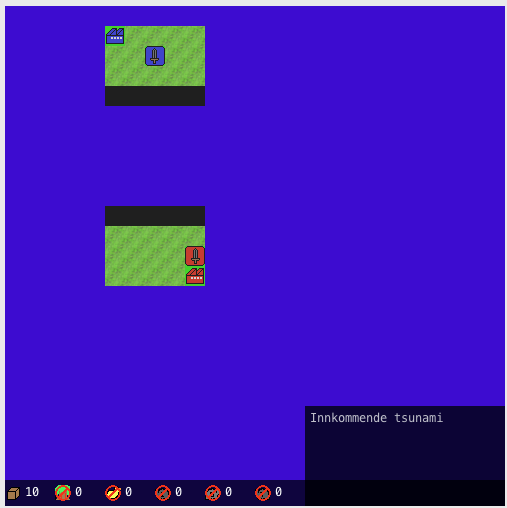
\includegraphics[scale=0.5]{images/Tsunami.png}}
\caption{Globale geohasarder kan oppstå som følge av mye global forsøpling, som for eksempel en tsunami.}
\label{fig:Tsunami}
\end{figure}

\begin{figure} 
\centering
\setlength\fboxsep{0.2pt}
\setlength\fboxrule{0.7pt}
\fbox{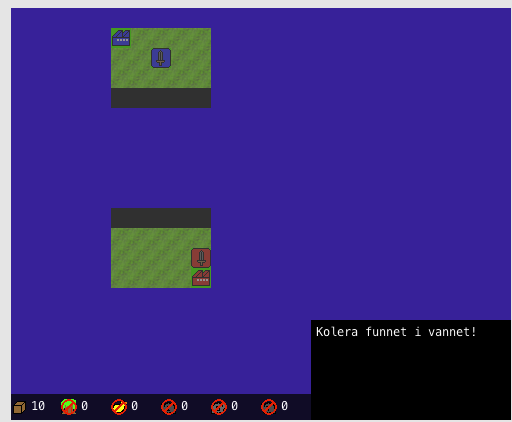
\includegraphics[scale=0.7]{images/Kolera.png}}
\caption{Lokale biohasarder kan oppstå som følge av mye lokal forurensning. Her er et sykdomsutbrudd.}
\label{fig:Kolera}
\end{figure}

\begin{figure} [H]
\centering
\setlength\fboxsep{0.2pt}
\setlength\fboxrule{0.7pt}
\fbox{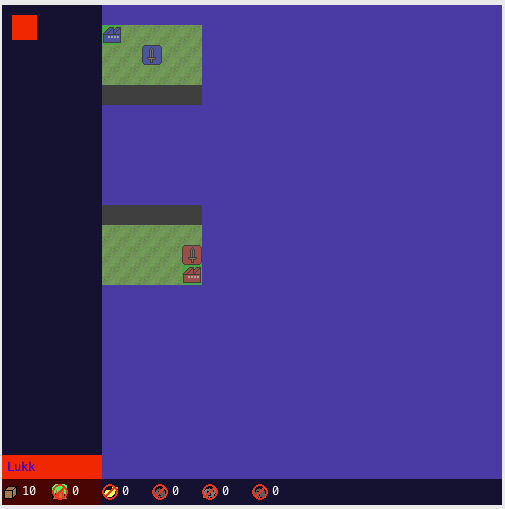
\includegraphics{images/OppgradereEnv.png}}
\caption{Miljøstasjonens effektivitet kan oppgraderes slik at den gjenvinner mer materialer fra hver avfallsenhet.}
\label{fig:OppgradereEnv}
\end{figure}

På figur~\ref{fig:OppgradereEnv} har den røde spilleren åpnet
oppgraderingsmenyen sin. Her har han mulighet til å oppgradere
effektiviteten av miljøstasjonen sin.

Legg merke til at disse skjermskuddene er tatt av en veldig tidlig
prototype som har hatt fokus på å implementere så mye av den tenkte
funksjonaliteten som mulig, heller enn å etablere et konsistent grafisk
uttrykk. Det var ønskelig å benytte så mye som mulig av den kode og
grafikk som ble til i vår tidlige prototype videre i den mer avanserte
prototypen\footnote{Noen vil kanskje si at dette ble gjort i tråd med
landsbyens filosofi om gjenbruk og gjenvinning.}. Mot en sluttfase vil
det være naturlig å erstatte eksempelgrafikken med noe grafikk som er
mer polert.


\cleardoublepage
\section{Avslutning}\label{sec:conclusion}
Denne seksjonen vil relatere prosjektet i forhold til spilldesign som
felt og diskutere spillets samfunnsnytte og forklare hva som er tenkt
rundt videre arbeid.

\subsection{Garbage Alert, i en større sammenheng}
Spillutforming på et generelt nivå starter ofte med en idè~\ref{bates},
eller en modifisering av et eksisterende konsept. Prosessen videre
varierer veldig fra utvikler til utvikler og selskap til selskap, men en
del fellestrekk finnes:
\begin{itemize}
\item Lage spillskisser
\item Definere spillbare elementer
\item Nivådesign
\item Innhold
\item Mekanikk
\end{itemize}
Etterhvert som denne prosessen går videre er det vanlig å dokumentere
alt i et designdokument. Dette dokumentet kan bli brukt som et rent
oppslagsverk for utviklere, og vil konstant være i endring. En felles
arbeidsflate for dette (en egen wiki eller lignende) blir også ofte brukt.

Måten Re³ designet Garbage Alert på, har klare trekk med den generelle
måten å drive spillutforming på. Etter at konseptet var unnfanget ble
det fokusert på å lage spillskisser, både av verdenen (øyene), og av
viktige elementer som miljøstasjonen. Det ble brukt mye tid på å finne
ut hvordan de ulike elementene skulle og burde interagere med hverandre.
Spillmekanikken ble utprøvd ved hjelp av en enkel prototype, noe som gav
verdifull tilbakemelding til den videre spillutformingen.

Om det er noe gruppen føler det burde ha gjort annerledes må det nok
være å lage en mer fullstendig prototype. Av erfaring viser dette seg å
ta ganske lang tid, og tidsaspektet for prosjektet var for kort.

\subsection{Spillets samfunnsnytte}
Garbage Alert har som mål å belyse nytten av gjenbruk og resirkulering, lokalt og globalt, gjennom et flerspiller dataspill (se seksjon \ref{sec:problemstilling}).

Gjenvinning av søppel står sentralt i Garbage Alert. Når spilleren gjenvinner ulike ressurser fra søppelet vil han/hun se at man ikke nødvendigvis er avhengig av å utvinne nye ressurser, men at man kan bruke ressursene man har på ny. Dette vil forhåpentligvis gi økt bevissthet rundt gjenbruk.

De ulike oppgraderingene som finnes i spillet kan relateres til forskning innen gjenbruk og resirkulering, som gjør det mulig å gjenbruke flere typer ressurser fra søppelet samt øke gjenvinningsgraden og effektiviteten. Dette har som mål å belyse hvor viktig det er å forske på disse aspektene rundt gjenbruk og nytten vi har av det.

Krig, som står sentralt i Garbage Alert, er ikke direkte en samfunnsnyttig del av spillet. Det er derimot flere aspekter med dette som kan relateres til dagens samfunn. De forskjellige mulighetene spilleren har innen bygging av forsvar og angrep viser at et økt gjenbruk (som ved å gi spilleren flere ressurser) gir muligheten til å bygge bedre bygninger, noe som må til for å vinne spillet. I tillegg til dette har katastrofene som kan inntreffe i spillet en parallell til dagens samfunn. Ved å ikke ta ansvar for søppelet, øker sannsynligheten for globale katastrofer, der global oppvarmning er et meget viktig tema idag. Noen av de geologiske katastrofene i spillet kan være et direkte resultat av global oppvarmning. De biologiske katastrofene er knyttet til mulige utfall dersom man ikke blir kvitt søppelet. I Garbage Alert finnes det både lokale og globale katastrofer, noe som er ment å belyse at både deg selv og andre blir berørt av handlinger som ikke nødvendigvis er utført av deg.

Katastrofene i spillet er i større grad en eksplisitt informativ konsekvens som belyser negative følger av dårlig håndtering av søppel. De fleste informative delene av spillet er derimot implisitte, og vil forhåpentligvis øke spillerens bevisshet rundt økt gjenbruk og nytten av dette. 

\subsection{Videre arbeid}
Et naturlig videre arbeid med Garbage Alert vil være å fullføre prototypen med implementasjon av flerspillerfunksjonalitet og ferdigstilt grafikk på mobile enheter. For å kunne fullføre prototypen burde minimum en designer og en programmerer ta del i prosjektet for å oppnå den samlede kompetansen som kreves. Ved ferdigstillelse av prototypen vil det være aktuelt å finne samarbeidspartnere som kan bidra med finansiering og markedsføring.

\cleardoublepage
\section{Oppsummering}
\emph{Garbage Alert} er spillet der du bestemmer verdens skjebne gjennom å gjenvinne og krige med med søppel. Gjennom å oppgradere sin miljøstasjon får man tilgang til forbedrede og nye metoder rundt gjenvinning, noe som gir spilleren muligheten til å avansere og til slutt gå av med seieren.  Geologiske og biologiske katastrofale hendelser oppstår som konsekvenser av krig med søppel og dårlige valg rundt gjenvinning. 
Spillet er utviklet av tre datastudenter, en geologistudent og en biologistudent ved NTNU. Deres tverrfaglighet og ulike egenskaper har gjennom en iterativ prosess skapt et konsept som de mener kan endre holdninger, opplyse om resirkulering, gjenvinning og dets konsekvenser gjennom et flerspiller-strategispill som sikter seg mot barn og unge mellom 10 og 17 år. 
Resultatet av deres arbeid er et spillkonsept og en prototype for mobile enheter. Konseptet tilrettelegger for muligheten for å danne en betaversjon av et underholdende og spennende spill med et morsomt audiovisuelt innhold. Adrenalinet av å være i krig med andre spillere, raske og ulike taktikker som overrasker de andre spillerne og plutselige katastrofer som kan snu spillet i alle retninger, er elementer som gjør \emph{Garbage Alert} til den neste mobilapplikasjonen alle snakker om. 

\thispagestyle{empty}
\bibliographystyle{apacite}
\bibliography{referanser}
\appendix \pagenumbering{roman} \pagestyle{plain}
\addcontentsline{toc}{section}{Appendiks}
\section{Prisliste} \label{A}

			\begin{figure} [H]
				\begin{center}
				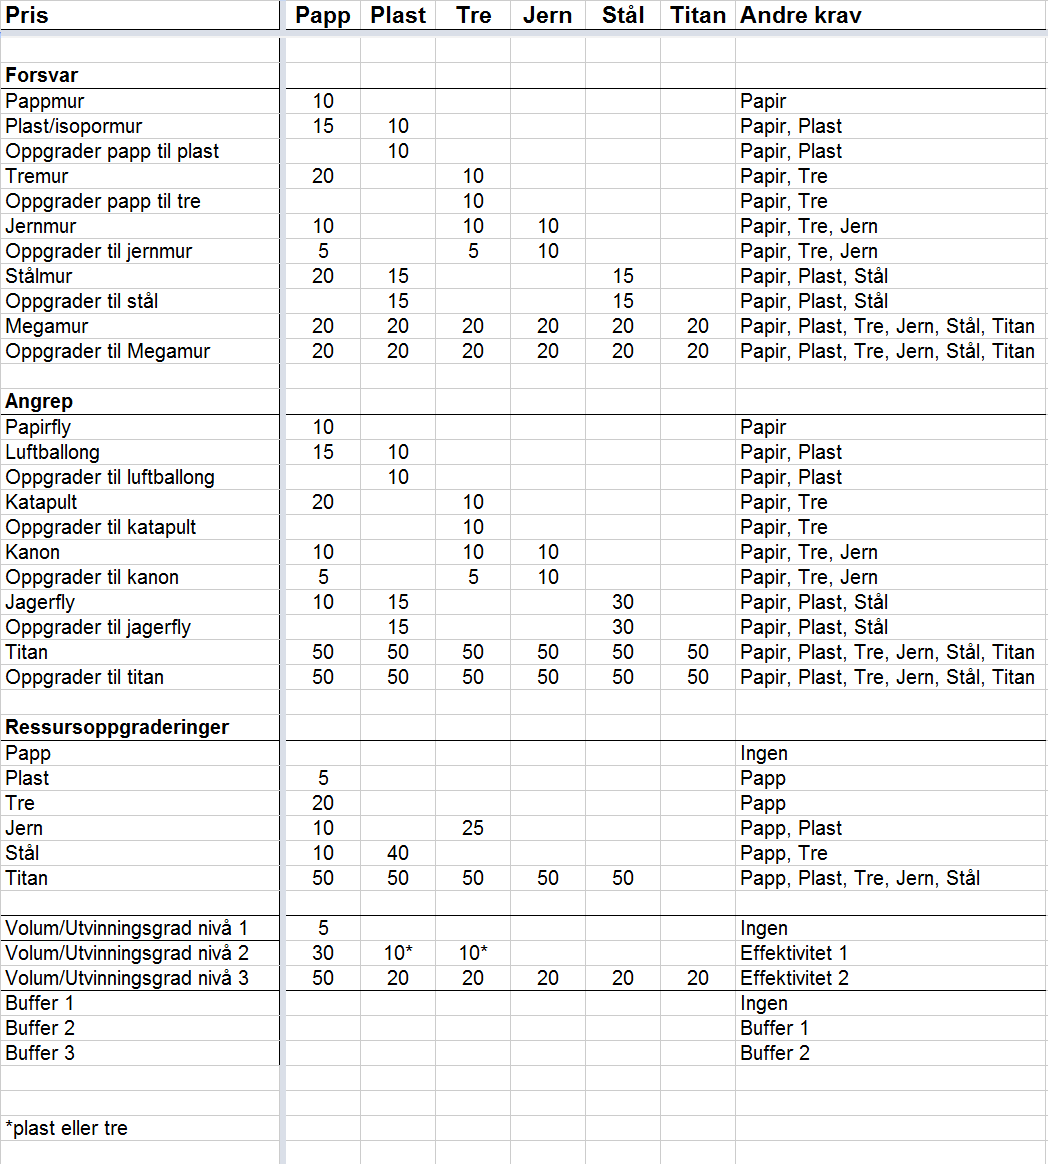
\includegraphics[width=155mm]{images/prisliste_stor}
				\caption{Utkast over prislite}
				\end{center}
			\end{figure}

\section{Helsepoeng og angrepsverdier} \label{B}

			\begin{figure} [H]
				\begin{center}
					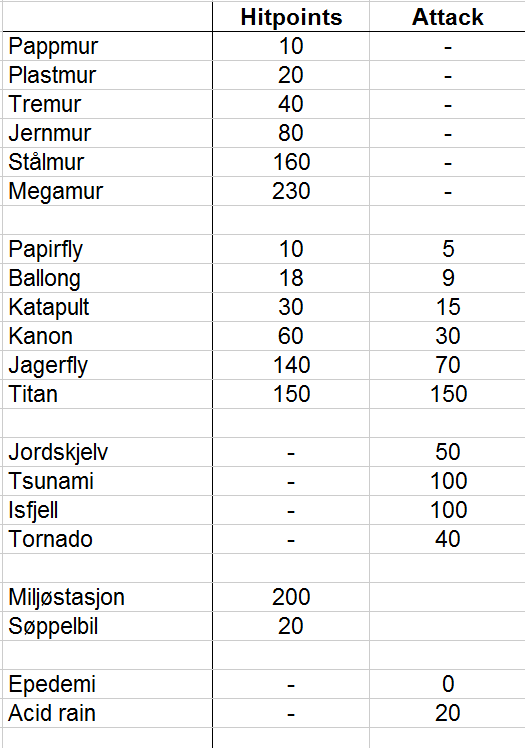
\includegraphics[width=77mm]{images/hitpoints_attack_stor}
				\end{center}
				\caption{Utkast over helsepoeng (hitpoints) og angrepsverdier (attack)}
			\end{figure}

\section{Gantt-diagram} \label{app:Gantt}
	\begin{figure} [H]
		\begin{center}
		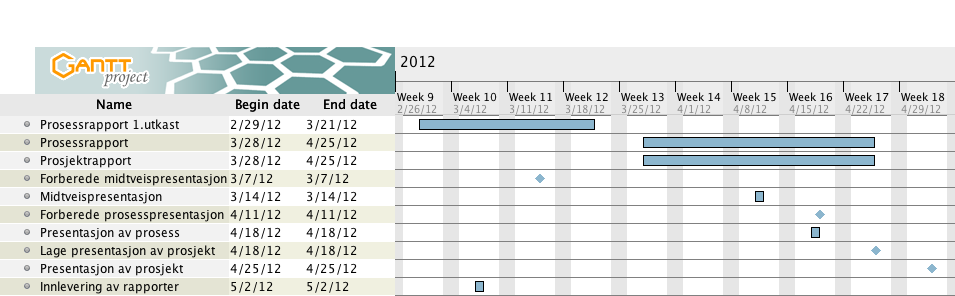
\includegraphics[width=\textwidth, angle=90]{images/EiTGantt}
		\caption{Gantt-diagram}
		\end{center}
	\end{figure}
\end{document}
